\subsection{ソフトウェア設計品質}

設計品質とは、設計がどのような性質を持つか、またその設計によって作られるソフトウェアがどのような品質を達成しやすいかに関する観点である。ここで扱う品質は、単に「よく動く」ことではなく、並行処理、イベント処理、永続化、分散、例外処理、統合、安全性、変動性など、多面的である。

\subsubsection{並行性}

\term{並行性}{Concurrency} は、複数の処理が同時または重なり合って進む性質である。設計では、処理をプロセス、タスク、スレッドなどの単位へどう分けるかを考える。

並行性の設計では、効率だけでなく、同期、排他制御、原子性、スケジューリングを考慮する必要がある。たとえば、複数の処理が同じデータを書き換える場合、順序が不適切だと結果が不安定になる。したがって、どのデータを共有するか、どこでロックするか、どの処理を非同期にするかを設計で明確にする。

\subsubsection{制御とイベント処理}

\term{制御}{Control} は、処理の流れをどう組み立てるかに関する設計である。\term{イベント処理}{Event Handling} は、利用者操作、外部メッセージ、タイマー、センサー入力などの出来事にどう反応するかに関する設計である。

イベント処理では、同期呼び出し、非同期メッセージ、コールバック、暗黙呼び出しなどの仕組みが使われる。反応型のシステムでは、イベント発生時の順序、重複、遅延、失敗時の扱いを設計しなければならない。

\subsubsection{データ永続化}

\term{データ永続化}{Data Persistence} は、プログラム終了後もデータを保持し、必要なときに取り出せるようにすることである。設計では、データベース、ファイル、キャッシュ、メッセージキュー、外部ストレージなどをどう使うかを決める。

永続化の設計では、保存形式、整合性、トランザクション、検索性能、バックアップ、復旧、権限管理を考慮する。データは長期に残るため、後から変更しにくい。したがって、データ構造は実装の都合だけでなく、将来の変更と保守を見越して決める必要がある。

\subsubsection{構成要素の分散}

\term{構成要素の分散}{Distribution of Components} は、ソフトウェア構成要素を複数のコンピュータ、ネットワーク、デバイスへ配置する設計である。分散させると、拡張性や可用性を高められる場合があるが、通信遅延、障害、整合性、監視、復旧が難しくなる。

分散設計では、構成要素間の通信方式、データ複製、障害時の再試行、サービス発見、負荷分散、セキュリティ境界を考える。特に、ネットワーク越しの呼び出しは、ローカル関数呼び出しとは違い、遅延や失敗が普通に起こる前提で設計する必要がある。

\subsubsection{誤り・例外処理と耐故障性}

\term{誤り処理}{Error Handling} と\term{例外処理}{Exception Handling} は、通常の処理から外れた状況をどう扱うかに関する設計である。\term{耐故障性}{Fault Tolerance} は、故障や誤りが起きても、影響を抑え、必要なサービスを続ける性質である。

設計では、どの異常を防ぐか、どの異常を検出するか、どの異常を許容するか、どの異常では停止するかを決める。例外を単に捕捉して無視すると、原因が隠れ、後で大きな障害になる。したがって、記録、通知、復旧、再試行、代替処理、停止条件を設計で明確にする。

\subsubsection{統合と相互運用性}

統合 は、複数の部品やシステムを組み合わせて一つの目的を達成することである。\term{相互運用性}{Interoperability} は、異なるシステムや構成要素がデータやサービスをやり取りして協調できる性質である。

この論点は、企業内システム、システムオブシステムズ、クラウドサービス連携、異なるフレームワークやライブラリを使う場合に重要である。設計では、データ形式、プロトコル、API、認証方式、エラー通知、バージョン互換性を決める。

\subsubsection{保証・セキュリティ・安全性}

\term{保証}{Assurance} は、ソフトウェアが意図どおりに動くという信頼を得ることに関わる。セキュリティ は、情報や資源を不正なアクセス、変更、破壊、利用不能化から守ることである。\term{安全性}{Safety} は、人命、財産、環境への危害を避けることである。

セキュリティ設計では、機密性、完全性、可用性、認証、認可、監査、攻撃時の被害限定、復旧を考える。安全性設計では、危険状態に至る条件、停止方法、警告、フェイルセーフ、冗長化を考える。どちらも後付けが難しいため、設計段階から扱う必要がある。

\subsubsection{変動性}

変動性 は、ソフトウェアに許されるバリエーションを扱う設計観点である。市場、利用組織、地域、法制度、設定、利用文脈によって、同じソフトウェアに異なる振る舞いや構成が求められることがある。

変動性は、ソフトウェア製品系列やシステムファミリで特に重要である。共通部分と可変部分を分ければ、複数の派生製品を効率よく作れる。フィーチャモデルは、機能や選択肢、その依存関係を整理するために使われる。

\par\smallskip
\begin{center}
\centering
\IfFileExists{assets/generated_figures/ch03/fig-ch03-06.png}{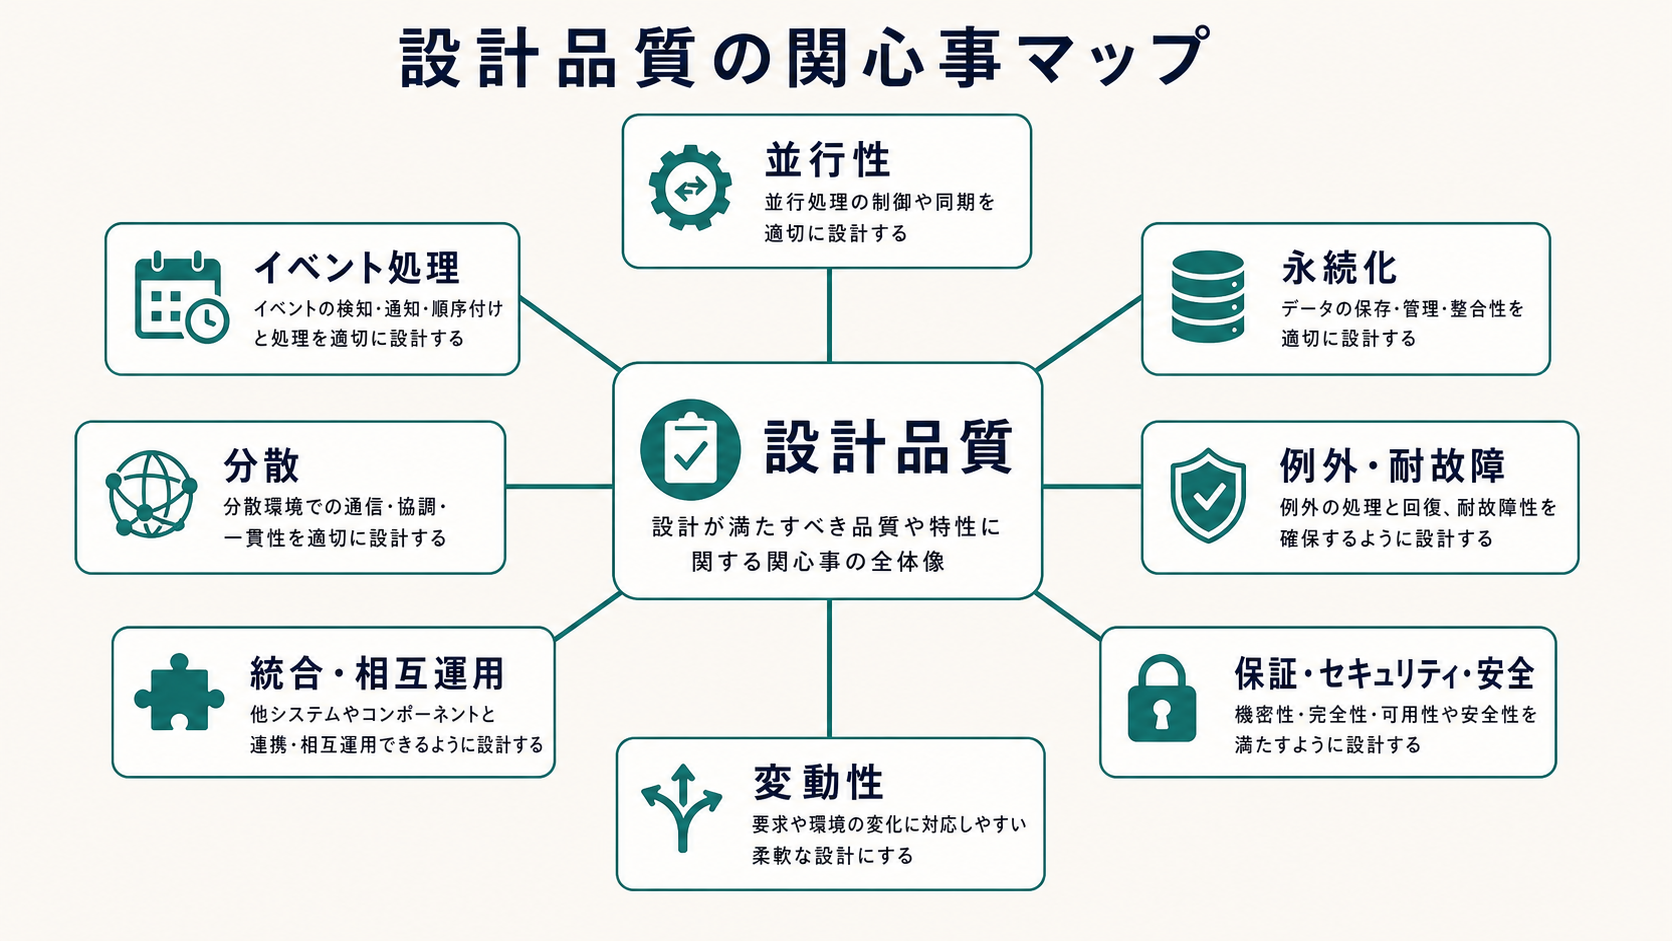
\includegraphics[width=0.96\linewidth]{assets/generated_figures/ch03/fig-ch03-06.png}}{\fbox{\parbox[c][48mm][c]{0.9\linewidth}{\centering 画像生成待ち\\設計品質の関心事マップ}}}
\par\smallskip
\refstepcounter{figure}\label{fig:ch03-06}図 \thefigure: 設計品質の関心事マップ
\end{center}
図 \thefigure は、設計品質の関心事マップを視覚的に整理したものである。
\par\smallskip
